\chapter{System Design and Implementation}\label{ch:implementation}
The system pipeline\footnote{See footnote on page~\pageref{foot:pipe}} consists of three separate processes:
data preprocessing~\ref{sec:data-preprocessing}, feature extraction~\ref{sec:feature-extraction} and
evaluation~\ref{sec:evaluation}.

The system is implemented in \textit{Python} programming language.
Libraries \textit{NumPy} and \textit{PyTorch} are being extensively used throughout the whole pipeline.

\section{Data Preprocessing}\label{sec:data-preprocessing}
\begin{wrapfigure}[7]{r}{0pt}
    \centering
    \raisebox{0pt}[\dimexpr\height-0.831\baselineskip\relax]{%
    \begin{forest}
        for tree={
        font=\ttfamily,
        grow'=0,
        child anchor=west,
        parent anchor=south,
        anchor=west,
        calign=first,
        edge path={
        \noexpand\path [draw, \forestoption{edge}]
        (!u.south west) +(7.5pt,0) |- node[fill,inner sep=1.25pt] {} (.child anchor)\forestoption{edge label};
        },
        before typesetting nodes={
        if n=1
        {insert before={[,phantom]}}
        {}
        },
        fit=band,
        before computing xy={l=15pt},
        }
        [dataset
        [name1
        [image1\_128x128.jpg]
        [image2\_128x128.jpg]
        [image3\_128x128.jpg]
        ]
        [name2
        [image1\_128x128.jpg]
        [image2\_128x128.jpg]
        ]
        [\ldots]
        ]
    \end{forest}
    }
    \caption{Standard image dataset format}
    \label{fig:dataset}
\end{wrapfigure}
The goal of preprocessing is to convert the input dataset~\ref{subsec:dataset-description} to a standard format.
The standardized dataset consists of directories with each directory representing one identity/label.
In these directories there are images corresponding to the identity.
In this case, the images contain faces in different positions.

The desired format is visualized in figure~\ref{fig:dataset}.

\subsection{Dataset Description}\label{subsec:dataset-description}
The input dataset consists of 15 videos and the same amount of annotation files in \textit{json}\footnote{An
open-standard file format that uses human-readable text to transmit data objects consisting of attribute–value pairs
and array data types.} format.

In every annotation file there is a dictionary object, where key is a name and value is a list of detections.
Every detection contains information about frame and the position of the face.
This information is used to transform the dataset to standardized format.
The reference face position was selected by human.
Because of that, the geometry of the area is not always consistent which significantly decreases the model performance.
For this reason, as is described in the following section~\ref{subsec:algorithm}, this reference position is not
used directly in the algorithm.

\subsection{Algorithm}\label{subsec:algorithm}
Before the presentation of the algorithm it is necessary to define "Intersection over Union (IoU)."
As the name implies IoU is computed as a fraction with intersection area in the numerator and union area in the
denominator (see figure~\ref{fig:iou}).

\begin{figure}[H]
    \centering
    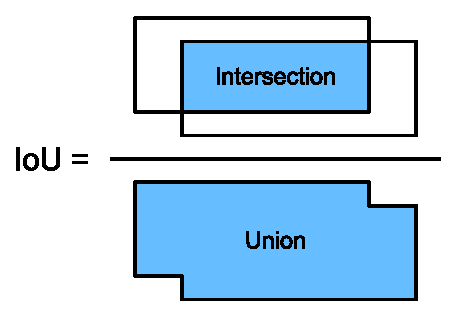
\includegraphics{images/implementation/iou.eps}
    \caption{IoU visualization\cite{IoU}}
    \label{fig:iou}
\end{figure}

The preprocessing algorithm consists of seven steps:
\begin{enumerate}
    \item First I iterate over the annotation files.
    \item Then I iterate over the names and detections within the file.
    \item In the third step I fetch the frame out of the video corresponding to the detection.
    \item Then I detect all the faces in the frame using MTCNN detector.
    The detector returns coordinates of the bounding boxes\footnote{A rectangle describing face position.} and the
    facial landmarks\footnote{Salient regions of the face.}.
    \item I select the detection which has the biggest "Intersection over Union (IoU)" with the bounding box from the
    annotation file.
    \item Now I perform face frontalization using the facial landmarks from the previous steps and the predetermined
    position of target facial landmarks.
    This is achieved by using the least squares method to find an affine transformation\footnote{A function between
    affine spaces which preserves points, straight lines and planes.} between the two sets of coordinates.
    After the transformation the image geometry is 128x128 and the facial landmarks are in the same position across
    the whole dataset.
    \item In the last step I save the transformed image on the path defined by the standardized dataset format
    (\path{dataset/name/image_128x128.jpg}).
\end{enumerate}

\section{Feature Extraction}\label{sec:feature-extraction}

\section{Evaluation}\label{sec:evaluation}

\begin{figure}[H]
    \centering
    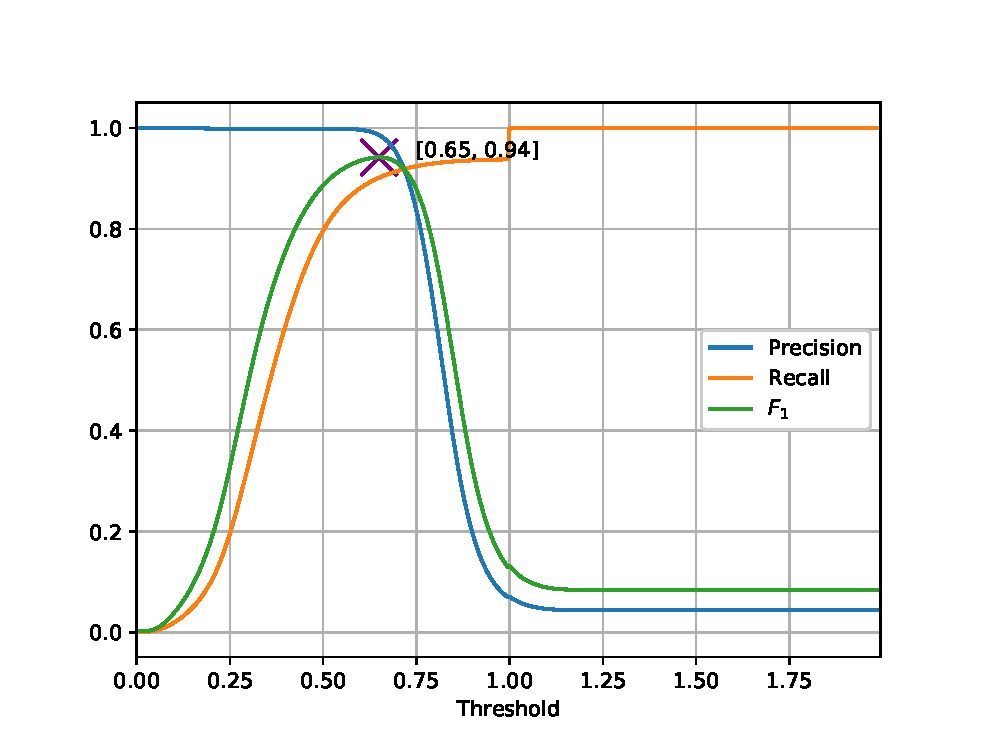
\includegraphics{images/implementation/prft_eyedea.eps}
    \caption{Progression of precision, recall and $F_1$ score with increasing thresholds values of the commercial
    system made bu Eyedea Recognition s. r. o.}
    \label{fig:prft_eyedea}
\end{figure}

\begin{figure}[H]
    \centering
    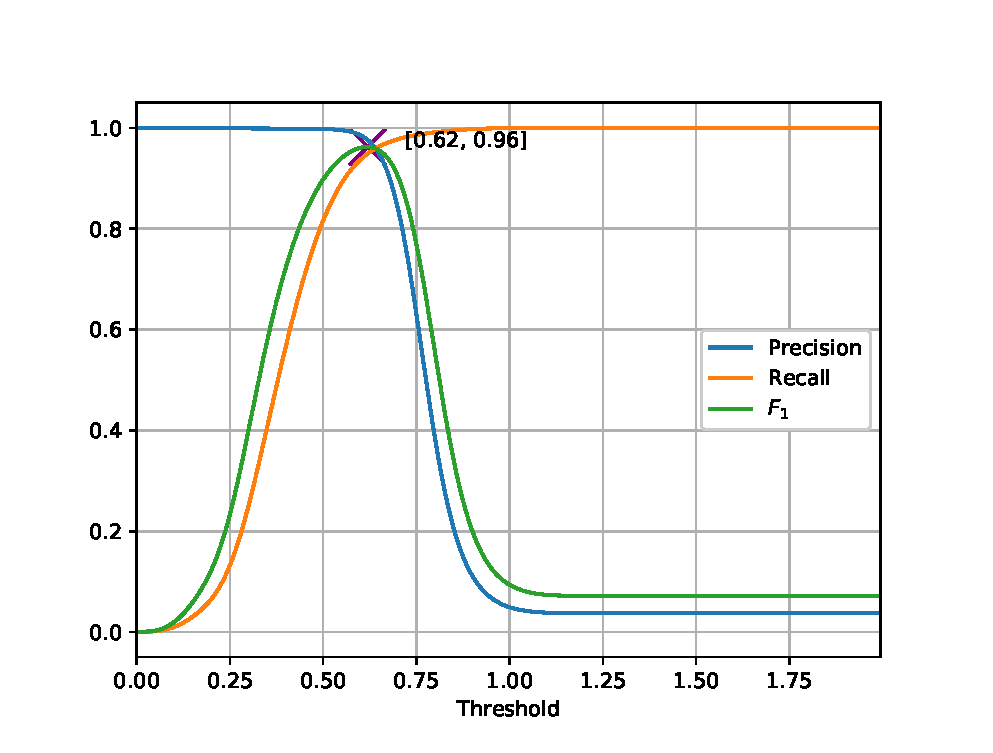
\includegraphics{images/implementation/prft_fav-128_N1.eps}
    \caption{Progression of precision, recall and $F_1$ score with increasing thresholds values}
    \label{fig:prft}
\end{figure}